


\begin{applicationActivities}

\begin{definition}
Let $T: V \rightarrow W$ be a linear transformation.  The \term{kernel} of $T$
is an important subspace of \(V\) defined by
\[
\ker T = \left\{ \vec{v} \in V\ \big|\ T(\vec{v})=\vec{z}\right\}
\]

\begin{center}
  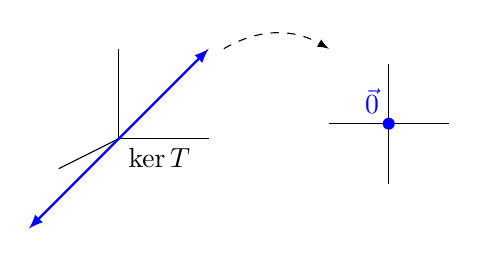
\begin{tikzpicture}[x=0.15in,y=0.15in]
    \begin{scope}[shift={(0,0)}]
      \draw (0,0) node[anchor=north west] {\(\ker T\)} -- (3,0);
      \draw (0,0) -- (0,3);
      \draw (0,0)  -- (-2,-1);
      \draw[thick,latex-latex,blue] (-3,-3) -- (3,3);
    \end{scope}
    \draw[dashed,-latex] (3.5,3) to [bend left=30] (7,3);
    \begin{scope}[shift={(9,0.5)}]
      \draw (-2,0) -- (2,0);
      \draw (0,-2) -- (0,2);
      \fill[blue] (0,0) circle (0.2)
            node[anchor=south east] {\(\vec{0}\)};
    \end{scope}
  \end{tikzpicture}
\end{center}
\end{definition}

\begin{activity}{5}
Let $T: \IR^2 \rightarrow \IR^3$ be given by
\[
  T\left(\begin{bmatrix}x \\ y \end{bmatrix} \right)
    =
  \begin{bmatrix} x \\ y \\ 0 \end{bmatrix}
    \hspace{3em}
    \text{with standard matrix }
  \begin{bmatrix} 1 & 0 \\ 0 & 1 \\ 0 & 0 \end{bmatrix}
\]
Which of these subspaces of \(\IR^2\) describes \(\ker T\),
the set of all vectors that transform into \(\vec 0\)?
\begin{enumerate}[a)]
\item \(\setBuilder{\begin{bmatrix}a \\ a\end{bmatrix}}{a\in\IR}\)
\item \(\setList{\begin{bmatrix}0\\0\end{bmatrix}}\)
\item \(\IR^2=\setBuilder{\begin{bmatrix}x \\ y\end{bmatrix}}{x,y\in\IR}\)
\end{enumerate}
\end{activity}

\begin{activity}{5}
Let $T: \IR^3 \rightarrow \IR^2$ be given by
\[
  T\left(\begin{bmatrix}x \\ y\\z \end{bmatrix} \right)
    =
  \begin{bmatrix} x \\ y \end{bmatrix}
    \hspace{3em}
    \text{with standard matrix }
  \begin{bmatrix} 1 & 0 & 0 \\ 0 & 1 & 0 \end{bmatrix}
\]
Which of these subspaces of \(\IR^3\) describes \(\ker T\),
the set of all vectors that transform into \(\vec 0\)?
\begin{multicols}{2}
\begin{enumerate}[a)]
\item \(\setBuilder{\begin{bmatrix}0 \\ 0\\ a\end{bmatrix}}{a\in\IR}\)
\item \(\setBuilder{\begin{bmatrix}a \\ a\\ 0\end{bmatrix}}{a\in\IR}\)
\item \(\setList{\begin{bmatrix}0\\0\\0\end{bmatrix}}\)
\item \(\IR^3=\setBuilder{\begin{bmatrix}x \\ y\\z\end{bmatrix}}{x,y,z\in\IR}\)
\end{enumerate}
\end{multicols}
\end{activity}

\begin{activity}{10}
Let $T: \IR^3 \rightarrow \IR^2$ be the linear transformation given by the
standard matrix
\[A=\begin{bmatrix} 3 & 4 & -1 \\ 1 & 2 & 1 \end{bmatrix}.\]
\begin{subactivity}
Set
\(
  T\left(\begin{bmatrix}x\\y\\z\end{bmatrix}\right)
    =
  \begin{bmatrix}
    \unknown+\unknown+\unknown \\
    \unknown+\unknown+\unknown
  \end{bmatrix}
    =
  \begin{bmatrix}0\\0\end{bmatrix}
\) to find a linear system of equations whose solution set is the kernel.
\end{subactivity}
\begin{subactivity}
Use $\RREF(A)$ to solve this homogeneous system of equations and find a basis
for the kernel of \(T\).
\end{subactivity}
\end{activity}


\begin{definition}
Let $T: V \rightarrow W$ be a linear transformation.
The \term{image} of $T$ is an important subspace of \(W\) defined by
\[
\Im T = \left\{ \vec{w} \in W\ \big|\ \text{there is some }\vec v\in V \text{ with } T(\vec{v})=\vec{w}\right\}
\]
In the examples below, the left example's image is all of \(\IR^2\), but the
right example's image is a planar subspace of \(\IR^3\).
\begin{center}
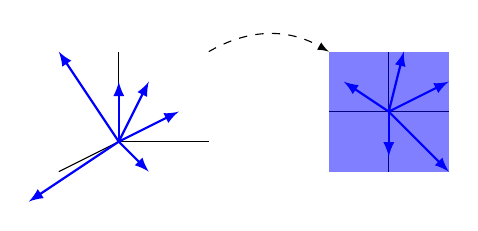
\begin{tikzpicture}[x=0.15in,y=0.15in]
  \begin{scope}[shift={(0,0)}]
    \draw (0,0) -- (3,0);
    \draw (0,0) -- (0,3);
    \draw (0,0) -- (-2,-1);
    \draw[thick,-latex,blue] (0,0) -- (2,1);
    \draw[thick,-latex,blue] (0,0) -- (1,2);
    \draw[thick,-latex,blue] (0,0) -- (0,2);
    \draw[thick,-latex,blue] (0,0) -- (1,-1);
    \draw[thick,-latex,blue] (0,0) -- (-2,3);
    \draw[thick,-latex,blue] (0,0) -- (-3,-2);
  \end{scope}
  \draw[dashed,-latex] (3,3) to [bend left=30] (7,3);
  \begin{scope}[shift={(9,1)}]
    \draw (-2,0) -- (2,0);
    \draw (0,-2) -- (0,2);
    \draw[thick,-latex,blue] (0,0) -- (0.5,2);
    \draw[thick,-latex,blue] (0,0) -- (2,1);
    \draw[thick,-latex,blue] (0,0) -- (-1.5,1);
    \draw[thick,-latex,blue] (0,0) -- (0,-1.5);
    \draw[thick,-latex,blue] (0,0) -- (2,-2);
    \fill[color=blue, opacity=0.5] (-2,-2) rectangle (2,2);
  \end{scope}
\end{tikzpicture}
\hspace{3em}
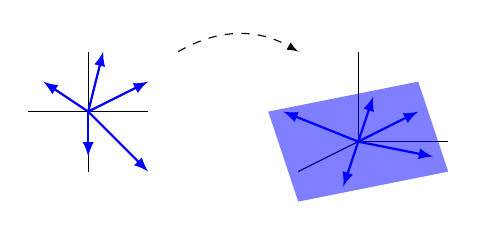
\begin{tikzpicture}[x=0.15in,y=0.15in]
  \begin{scope}[shift={(0,1)}]
    \draw (-2,0) -- (2,0);
    \draw (0,-2) -- (0,2);
    \draw[thick,-latex,blue] (0,0) -- (0.5,2);
    \draw[thick,-latex,blue] (0,0) -- (2,1);
    \draw[thick,-latex,blue] (0,0) -- (-1.5,1);
    \draw[thick,-latex,blue] (0,0) -- (0,-1.5);
    \draw[thick,-latex,blue] (0,0) -- (2,-2);
  \end{scope}
  \draw[dashed,-latex] (3,3) to [bend left=30] (7,3);
  \begin{scope}[shift={(9,0)}]
    \draw (0,0) -- (3,0);
    \draw (0,0) -- (0,3);
    \draw (0,0) -- (-2,-1);
    \draw[thick,-latex,blue] (0,0) -- (0.5,1.5);
    \draw[thick,-latex,blue] (0,0) -- (2,1);
    \draw[thick,-latex,blue] (0,0) -- (-2.5,1);
    \draw[thick,-latex,blue] (0,0) -- (-0.5,-1.5);
    \draw[thick,-latex,blue] (0,0) -- (2.5,-0.5);
    \fill[color=blue, opacity=0.5] (-2,-2) -- (3,-1) -- (2,2) -- (-3,1) -- (-2,-2);
  \end{scope}
\end{tikzpicture}
\end{center}
\end{definition}

\begin{activity}{5}
Let $T: \IR^2 \rightarrow \IR^3$ be given by
\[
  T\left(\begin{bmatrix}x \\ y \end{bmatrix} \right)
    =
  \begin{bmatrix} x \\ y \\ 0 \end{bmatrix}
    \hspace{3em}
    \text{with standard matrix }
  \begin{bmatrix} 1 & 0 \\ 0 & 1 \\ 0 & 0 \end{bmatrix}
\]
Which of these subspaces of \(\IR^3\) describes \(\Im T\),
the set of all vectors that are the result of using \(T\) to transform
\(\IR^2\) vectors?
\begin{multicols}{2}
\begin{enumerate}[a)]
\item \(\setBuilder{\begin{bmatrix}0 \\ 0\\ a\end{bmatrix}}{a\in\IR}\)
\item \(\setBuilder{\begin{bmatrix}a \\ b\\ 0\end{bmatrix}}{a,b\in\IR}\)
\item \(\setList{\begin{bmatrix}0\\0\\0\end{bmatrix}}\)
\item \(\IR^3=\setBuilder{\begin{bmatrix}x \\ y\\z\end{bmatrix}}{x,y,z\in\IR}\)
\end{enumerate}
\end{multicols}
\end{activity}

\begin{activity}{5}
Let $T: \IR^3 \rightarrow \IR^2$ be given by
\[
  T\left(\begin{bmatrix}x \\ y\\z \end{bmatrix} \right)
    =
  \begin{bmatrix} x \\ y \end{bmatrix}
    \hspace{3em}
    \text{with standard matrix }
  \begin{bmatrix} 1 & 0 & 0 \\ 0 & 1 & 0 \end{bmatrix}
\]
Which of these subspaces of \(\IR^2\) describes \(\Im T\),
the set of all vectors that are the result of using \(T\) to transform
\(\IR^3\) vectors?
\begin{enumerate}[a)]
\item \(\setBuilder{\begin{bmatrix}a \\ a\end{bmatrix}}{a\in\IR}\)
\item \(\setList{\begin{bmatrix}0\\0\end{bmatrix}}\)
\item \(\IR^2=\setBuilder{\begin{bmatrix}x \\ y\end{bmatrix}}{x,y\in\IR}\)
\end{enumerate}
\end{activity}


\begin{activity}{5}
Let $T: \IR^4 \rightarrow \IR^3$ be the linear transformation given by the
standard matrix
\[
  A
    =
  \begin{bmatrix} 3 & 4 & 7 & 1\\ -1 & 1 & 0 & 2 \\ 2 & 1 & 3 & -1 \end{bmatrix}
    =
  \begin{bmatrix}T(\vec e_1)&T(\vec e_2)&T(\vec e_3)&T(\vec e_4)\end{bmatrix}
.\]

Since \(T(\vec v)=T(x_1\vec e_1+x_2\vec e_2+x_3\vec e_3+x_4\vec e_4)\),
the set of vectors
\[
  \setList{
    \begin{bmatrix}3\\-1\\2\end{bmatrix},
    \begin{bmatrix}4\\1\\1\end{bmatrix},
    \begin{bmatrix}7\\0\\3\end{bmatrix},
    \begin{bmatrix}1\\2\\-1\end{bmatrix}
  }
\]
\begin{enumerate}[a)]
\item spans \(\Im T\)
\item is a linearly independent subset of \(\Im T\)
\item is a basis for \(\Im T\)
\end{enumerate}
\end{activity}


\begin{observation}
Let $T: \IR^4 \rightarrow \IR^3$ be the linear transformation given by the
standard matrix
\[
  A
    =
  \begin{bmatrix} 3 & 4 & 7 & 1\\ -1 & 1 & 0 & 2 \\ 2 & 1 & 3 & -1 \end{bmatrix}
.\]

Since the set
\(
  \setList{
    \begin{bmatrix}3\\-1\\2\end{bmatrix},
    \begin{bmatrix}4\\1\\1\end{bmatrix},
    \begin{bmatrix}7\\0\\3\end{bmatrix},
    \begin{bmatrix}1\\2\\-1\end{bmatrix}
  }
\)
spans \(\Im T\), we can obtain a basis for \(\Im T\) by finding
\(
  \RREF A
    =
  \begin{bmatrix} 1 & 0 & 1 & -1\\ 0 & 1 & 1 & 1 \\ 0 & 0 & 0 & 0 \end{bmatrix}
\)
and only using the vectors corresponding to pivot columns:
\[
  \setList{
    \begin{bmatrix}3\\-1\\2\end{bmatrix},
    \begin{bmatrix}4\\1\\1\end{bmatrix}
  }
\]
\end{observation}

\begin{fact}
Let  $T:\IR^n\to\IR^m$ be a linear transformation with standard matrix $A$.

\begin{itemize}
\item The kernel of \(T\) is the solution set of the homogeneous system given
by the augmented matrix $\begin{bmatrix}[c|c]A&\vec 0\end{bmatrix}$.
Use the coefficients of its free variables to get a basis for the kernel.
\item The image of \(T\) is the span of the columns of \(A\). Remove
the vectors creating non-pivot columns in \(\RREF A\) to get a basis
for the image.
\end{itemize}
\end{fact}


\begin{activity}{10}
Let $T: \IR^3 \rightarrow \IR^4$ be the linear transformation given by the
standard matrix
\[
  A
    =
  \begin{bmatrix} 1 & -3 & 2\\ 2 & -6 & 0 \\ 0 & 0 & 1 \\ -1 & 3 & 1 \end{bmatrix}
.\]

Find a basis for the kernel and a basis for the image of \(T\).
\end{activity}
\begin{definition}
Let $T: V \rightarrow W$ be a linear transformation.
$T$ is called \term{injective} or \term{one-to-one} if $T$ does not map two
distinct vectors to the same place.  More precisely, $T$ is injective if
$T(\vec{v}) \neq T(\vec{w})$ whenever $\vec{v} \neq \vec{w}$.

\begin{center}
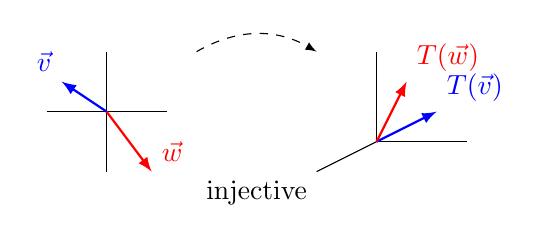
\begin{tikzpicture}[x=0.15in,y=0.15in]
  \begin{scope}[shift={(0,1)}]
    \draw (-2,0) -- (2,0);
    \draw (0,-2) -- (0,2);
    \draw[thick,-latex,blue] (0,0) -- (-1.5,1)
          node[anchor=south east] {\(\vec v\)};
    \draw[thick,-latex,red] (0,0) -- (1.5,-2)
          node[anchor=south west] {\(\vec w\)};
  \end{scope}
  \draw[dashed,-latex] (3,3) to [bend left=30] (7,3);
  \begin{scope}[shift={(9,0)}]
    \draw (0,0) -- (3,0);
    \draw (0,0) -- (0,3);
    \draw (0,0) -- (-2,-1);
    \draw[thick,-latex,blue] (0,0) -- (2,1)
          node[anchor=south west] {\(T(\vec v)\)};
    \draw[thick,-latex,red] (0,0) -- (1,2)
          node[anchor=south west] {\(T(\vec w)\)};
  \end{scope}
  \node[anchor=north] at (5,-1) {injective};
\end{tikzpicture}
\hspace{3em}
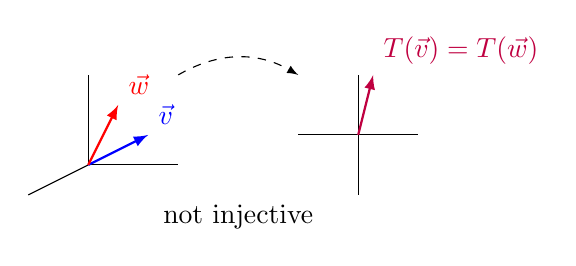
\begin{tikzpicture}[x=0.15in,y=0.15in]
  \begin{scope}[shift={(0,0)}]
    \draw (0,0) -- (3,0);
    \draw (0,0) -- (0,3);
    \draw (0,0) -- (-2,-1);
    \draw[thick,-latex,blue] (0,0) -- (2,1)
          node[anchor=south west] {\(\vec v\)};
    \draw[thick,-latex,red] (0,0) -- (1,2)
          node[anchor=south west] {\(\vec w\)};
  \end{scope}
  \draw[dashed,-latex] (3,3) to [bend left=30] (7,3);
  \begin{scope}[shift={(9,1)}]
    \draw (-2,0) -- (2,0);
    \draw (0,-2) -- (0,2);
    \draw[thick,-latex,purple] (0,0) -- (0.5,2)
          node[anchor=south west] {\(T(\vec v)=T(\vec w)\)};
  \end{scope}
  \node[anchor=north] at (5,-1) {not injective};
\end{tikzpicture}
\end{center}
\end{definition}

\begin{activity}{3}
Let $T: \IR^3 \rightarrow \IR^2$ be given by
\[
  T\left(\begin{bmatrix}x \\ y\\z \end{bmatrix} \right)
    =
  \begin{bmatrix} x \\ y \end{bmatrix}
    \hspace{3em}
    \text{with standard matrix }
  \begin{bmatrix} 1 & 0 & 0 \\ 0 & 1 & 0 \end{bmatrix}
\]
Is \(T\) injective?
\begin{enumerate}[a)]
\item Yes, because \(T(\vec v)=T(\vec w)\) whenever \(\vec v=\vec w\).
\item Yes, because \(T(\vec v)\not=T(\vec w)\) whenever \(\vec v\not=\vec w\).
\item No, because 
  \(
    T\left(\begin{bmatrix}0\\0\\1\end{bmatrix}\right)
      \not=
    T\left(\begin{bmatrix}0\\0\\2\end{bmatrix}\right)
  \)
\item No, because 
  \(
    T\left(\begin{bmatrix}0\\0\\1\end{bmatrix}\right)
      =
    T\left(\begin{bmatrix}0\\0\\2\end{bmatrix}\right)
  \)
\end{enumerate}
\end{activity}

\begin{activity}{2}
Let $T: \IR^2 \rightarrow \IR^3$ be given by
\[
  T\left(\begin{bmatrix}x \\ y \end{bmatrix} \right)
    =
  \begin{bmatrix} x \\ y \\ 0 \end{bmatrix}
    \hspace{3em}
    \text{with standard matrix }
  \begin{bmatrix} 1 & 0 \\ 0 & 1 \\ 0 & 0 \end{bmatrix}
\]
\begin{enumerate}[a)]
\item Yes, because \(T(\vec v)=T(\vec w)\) whenever \(\vec v=\vec w\).
\item Yes, because \(T(\vec v)\not=T(\vec w)\) whenever \(\vec v\not=\vec w\).
\item No, because 
  \(
    T\left(\begin{bmatrix}1\\2\end{bmatrix}\right)
      \not=
    T\left(\begin{bmatrix}3\\4\end{bmatrix}\right)
  \)
\item No, because 
  \(
    T\left(\begin{bmatrix}1\\2\end{bmatrix}\right)
      =
    T\left(\begin{bmatrix}3\\4\end{bmatrix}\right)
  \)
\end{enumerate}
\end{activity}

\begin{definition}
Let $T: V \rightarrow W$ be a linear transformation.
$T$ is called \term{surjective} or \term{onto} if every element of $W$ is mapped to by an element of $V$.  More precisely, for every $\vec{w} \in W$, there is some $\vec{v} \in V$ with $T(\vec{v})=\vec{w}$.
\begin{center}
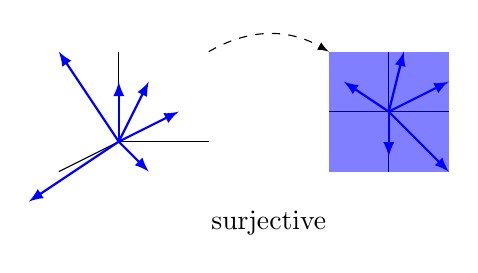
\begin{tikzpicture}[x=0.15in,y=0.15in]
  \begin{scope}[shift={(0,0)}]
    \draw (0,0) -- (3,0);
    \draw (0,0) -- (0,3);
    \draw (0,0) -- (-2,-1);
    \draw[thick,-latex,blue] (0,0) -- (2,1);
    \draw[thick,-latex,blue] (0,0) -- (1,2);
    \draw[thick,-latex,blue] (0,0) -- (0,2);
    \draw[thick,-latex,blue] (0,0) -- (1,-1);
    \draw[thick,-latex,blue] (0,0) -- (-2,3);
    \draw[thick,-latex,blue] (0,0) -- (-3,-2);
  \end{scope}
  \draw[dashed,-latex] (3,3) to [bend left=30] (7,3);
  \begin{scope}[shift={(9,1)}]
    \draw (-2,0) -- (2,0);
    \draw (0,-2) -- (0,2);
    \draw[thick,-latex,blue] (0,0) -- (0.5,2);
    \draw[thick,-latex,blue] (0,0) -- (2,1);
    \draw[thick,-latex,blue] (0,0) -- (-1.5,1);
    \draw[thick,-latex,blue] (0,0) -- (0,-1.5);
    \draw[thick,-latex,blue] (0,0) -- (2,-2);
    \fill[color=blue, opacity=0.5] (-2,-2) rectangle (2,2);
  \end{scope}
  \node[anchor=north] at (5,-2) {surjective};
\end{tikzpicture}
\hspace{3em}
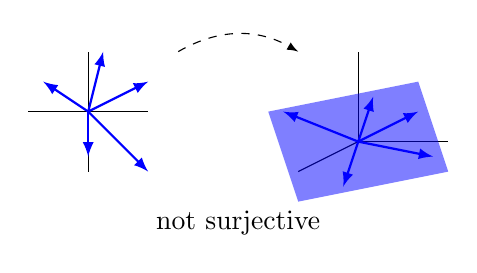
\begin{tikzpicture}[x=0.15in,y=0.15in]
  \begin{scope}[shift={(0,1)}]
    \draw (-2,0) -- (2,0);
    \draw (0,-2) -- (0,2);
    \draw[thick,-latex,blue] (0,0) -- (0.5,2);
    \draw[thick,-latex,blue] (0,0) -- (2,1);
    \draw[thick,-latex,blue] (0,0) -- (-1.5,1);
    \draw[thick,-latex,blue] (0,0) -- (0,-1.5);
    \draw[thick,-latex,blue] (0,0) -- (2,-2);
  \end{scope}
  \draw[dashed,-latex] (3,3) to [bend left=30] (7,3);
  \begin{scope}[shift={(9,0)}]
    \draw (0,0) -- (3,0);
    \draw (0,0) -- (0,3);
    \draw (0,0) -- (-2,-1);
    \draw[thick,-latex,blue] (0,0) -- (0.5,1.5);
    \draw[thick,-latex,blue] (0,0) -- (2,1);
    \draw[thick,-latex,blue] (0,0) -- (-2.5,1);
    \draw[thick,-latex,blue] (0,0) -- (-0.5,-1.5);
    \draw[thick,-latex,blue] (0,0) -- (2.5,-0.5);
    \fill[color=blue, opacity=0.5] (-2,-2) -- (3,-1) -- (2,2) -- (-3,1) -- (-2,-2);
  \end{scope}
  \node[anchor=north] at (5,-2) {not surjective};
\end{tikzpicture}
\end{center}
\end{definition}

\begin{activity}{3}
Let $T: \IR^2 \rightarrow \IR^3$ be given by
\[
  T\left(\begin{bmatrix}x \\ y \end{bmatrix} \right)
    =
  \begin{bmatrix} x \\ y \\ 0 \end{bmatrix}
    \hspace{3em}
    \text{with standard matrix }
  \begin{bmatrix} 1 & 0 \\ 0 & 1 \\ 0 & 0 \end{bmatrix}
\]
Is \(T\) surjective?
\begin{enumerate}[a)]
\item Yes, because for every \(\vec w=\begin{bmatrix}x\\y\\z\end{bmatrix}\in\IR^3\),
there exists \(\vec v=\begin{bmatrix}x\\y\end{bmatrix}\in\IR^2\) such that
\(T(\vec v)=\vec w\).
\item No, because 
  \(
    T\left(\begin{bmatrix}x\\y\end{bmatrix}\right)
  \)
can never equal
  \(
  \begin{bmatrix} 1 \\ 1 \\ 1 \end{bmatrix}
  \).
\item No, because 
  \(
    T\left(\begin{bmatrix}x\\y\end{bmatrix}\right)
  \)
can never equal
  \(
  \begin{bmatrix} 0 \\ 0 \\ 0 \end{bmatrix}
  \).
\end{enumerate}
\end{activity}

\begin{activity}{2}
Let $T: \IR^3 \rightarrow \IR^2$ be given by
\[
  T\left(\begin{bmatrix}x \\ y\\z \end{bmatrix} \right)
    =
  \begin{bmatrix} x \\ y \end{bmatrix}
    \hspace{3em}
    \text{with standard matrix }
  \begin{bmatrix} 1 & 0 & 0 \\ 0 & 1 & 0 \end{bmatrix}
\]
Is \(T\) surjective?
\begin{enumerate}[a)]
\item Yes, because for every \(\vec w=\begin{bmatrix}x\\y\end{bmatrix}\in\IR^2\),
there exists \(\vec v=\begin{bmatrix}x\\y\\42\end{bmatrix}\in\IR^3\) such that
\(T(\vec v)=\vec w\).
\item Yes, because for every \(\vec w=\begin{bmatrix}x\\y\end{bmatrix}\in\IR^2\),
there exists \(\vec v=\begin{bmatrix}0\\0\\z\end{bmatrix}\in\IR^3\) such that
\(T(\vec v)=\vec w\).
\item No, because 
  \(
    T\left(\begin{bmatrix}x\\y\\z\end{bmatrix}\right)
  \)
can never equal
  \(
  \begin{bmatrix} 3\\-2 \end{bmatrix}
  \).
\end{enumerate}
\end{activity}

\begin{observation}
As we will see, it's no coincidence that the \(\RREF\) of the
injective map's standard matrix
\[
  \begin{bmatrix} 1 & 0 \\ 0 & 1 \\ 0 & 0 \end{bmatrix}
\]
has all pivot columns. Similarly, the \(\RREF\) of the surjective map's
standard matrix
\[
  \begin{bmatrix} 1 & 0 & 0 \\ 0 & 1 & 0 \end{bmatrix}
\]
has a pivot in each row.
\end{observation}



\end{applicationActivities}
